\section{Information theory quantifiers}\label{sec:quanti}

Systems that evolve over time are called dynamical systems.
Generally, only measurements of scalar time series $X(t)$ are accessible, these time series may be function of variables $V=\{ v_1, v_2,\cdots, v_k\}$ describing the underlying dynamics (i.e. $dV/dt=f(V)$).
The goal is to infer properties and reach conclusions of an unknown system from the analysis of measured record of observational data.
The key question would be to know how much information about the dynamics of the underlying processes can be revealed by the analyzed data.
A probability distribution function (PDF) $P$ is typically used to quantify the apportionment of a time series $X(t)$.
Information Theory quantifiers can be defined as measures that characterize properties of the PDF associated with these time series, they allow to extract information about the studied system.
We can see these quantifiers as metrics in the PDFs space, they enable to compare and classify different sets of data according to their PDFs where stochastic and deterministic are the two extremes of processes.

Here, we are concerned in chaotic dynamics, which are fundamentally \textit{causal} and \textit{statistical} in nature.
For this reason, we are forced to use a different approach since a purely statistical approach ignores the correlations between successive values from the time series; and a causal approach focuses on the PDFs of data sequences.

The selected quantifiers are based on symbolic counting and ordinal pattern statistics.
They make it possible to distinguish between the two main features: the \textit{information content} of data and their \textit{complexity}.
It is important to highlight that rather than referring to a physical space, here we talk about a space of probability density functions.

In this section, we will introduce Information Theory quantifiers defined over discrete PDFs since discrete time series is our scope.
Nevertheless, in \cite{Shannon1948} definitions for the continuous case can be found. 

\subsection{Shannon entropy and statistical complexity}

Entropy is a measure of the uncertainty associated with a physical process that is described by $P$.
The Shannon entropy is considered as the most natural one \cite{Shannon1948} when dealing with information content.

Let define a discrete probability distribution $P=\{p_i; i=1,\ldots, N\}$ with $\sum_{i=1}^N p_i = 1$, were $N$ is the number of possible states of the system under study.
Then, Shannon's logarithmic information measure:
\begin{equation}
\label{Shannon-disc}
S[P] ~=~ -\sum_{i=1}^{N} p_i \ln \left[ p_i \right] \
\end{equation}

When $S[P] = S_{\min} = 0$, the prediction of which outcome $i$ will occur is a complete certainty.
In this case, it is maximal the knowledge of the underlying process described by the probability distribution.
On the contrary, we have minimal knowledge in a case of a uniform distribution $P_e = \{ p_i = 1/N; i=1, \ldots , N \}$ since every outcome has the same probability of occurrence, and the uncertainty is maximal, i.e., $S[P_e] = S_{\max} = \ln N$.
These two situations are extreme cases, therefore we focus on the `normalized' Shannon entropy, $0 \leq H \leq 1$, given as
\begin{equation}
\label{shannon-disc-normalizada}
H[P] = S[P] / S_{\max} \
\end{equation}

On the other hand, there is not a unique definition of the concept of complexity.
In this paper, the aim is to describe the complexity of the time series rather than that of the underlying systems.
As stated by Kantz \cite{Kantz1998}, complex data might be generated by ``simple" systems, while ``complicated" models can generate low complexity outputs.
A quantitative complexity can be defined as a measure that assigns low values both to uncorrelated random data (maximal Shannon entropy) and also to perfectly ordered data (null Shannon entropy).
Then, if we have an ordered sequence, such as a simple oscillation or trend, the statistical complexity would be low, and the same would happen with an unordered sequence, such as uncorrelated white noise.
In the middle of this situation the characterization of data is more difficult hence the complexity would be higher.

We look forward a quantifier functional of a PDF, $C[P]$, in order to measure the degree  of complexity or of correlational structures.  
As depicted in \cite{Feldman2008} the functional is relate to organization, correlational structure, memory, regularity, symmetry, patterns, and other properties.

Rosso and coworkers \cite{Lamberti2004} introduced a suitable \textit{Statistical Complexity Measure} (SCM) $C$, that is  based on the seminal notion advanced by L\'opez-Ruiz {\it et al.} \cite{Lopez-Ruiz1995}.
SCM is defined as the product of a measure of information and a measure of disequilibrium  and it is able to detect the distance from the equiprobable distribution of the accessible states.

This statistical complexity measure \cite{Martin2003,Lamberti2004} is defined as follows: 
\begin{equation}
C[P] = Q_{J}[P,P_e] \cdot H[P]
\label{complexity}
\end{equation}
$H$ is the normalized Shannon entropy, see eq. \ref{shannon-disc-normalizada}, and $Q_{J}$ is the disequilibrium  defined in terms of the Jensen-Shannon divergence $J[P, P_e]$, \cite{Grosse2002}.
That is,
\begin{equation}
\label{disequilibrium}	
Q_{J} [ P, P_e] = Q_{0} J[ P, P_e] = Q_{0} \{ S[(P + P_e)/2 ] - S[ P ]/2 - S[P_e]/2\}
\end{equation}
$Q_0$ is a normalization constant such that $0 \leq Q_{J} \leq 1$:
\begin{equation}
Q_0 ~=~ -2 \left\{ {\frac{N+1}{N}} \ln (N+1) - \ln (2N) + \ln N \right\}^{-1} \
\label{q0-jensen-1}
\end{equation}
This value is obtained in a totally deterministic situation, where only one components of $P$ has a no null value equal to one.

Note that the above introduced SCM depends on two different probability distributions: one associated with the system under analysis, $P$, and the other with the uniform distribution, $P_e$.
Furthermore, it was shown that for a given value of $H$, the range of possible $C$ values varies between a minimum $C_{min}$ and a maximum $C_{max}$, restricting the possible values of the SCM \cite{Martin2006}.
Thus, it is clear that important additional information related to the correlational structure between the components of the physical system is provided by evaluating the statistical complexity measure. 

\subsection{Determination of a probability distribution}

The evaluation derived from the  Information Theory quantifiers suppose some prior knowledge about the system; specifically for those previously introduced (Shannon entropy and statistical complexity), a probability distribution associated to the time series under analysis should be provided before.
The determination of the most adequate PDF is a fundamental problem because the PDF $P$ and the sample space $\Omega$ are inextricably linked.
Usual methodologies assign to each value of the series $X(t)$ (or non-overlapped set of consecutive values) a symbol from a finite alphabet $A=\{a_1,\dots,a_M\}$, thus creating a {\it symbolic sequence} that can be regarded to as a {\it non causal coarse grained\/} description of the time series under consideration. 
In this case, information on the dynamics of the system is lost, such as order relations and the time scales.

If we want to incorporate {\it Causal information\/} we have to add information about the past dynamics of the system, this is done by the assignment of symbols of alphabet $A$ to a portion of the trajectory.
The Bandt and Pompe (BP) \cite{Bandt2002} method is a simple and robust methodology that compares neighboring values in a time series and, thus solves this issue.
The causality property of the PDF allows quantifiers (based on this PDFs) to discriminate between deterministic and stochastic systems \cite{Rosso2007B}.
The steps are, first it is needed to create  symbolic data by ranking the values of the series; and second to define by reordering the embedded data in ascending order.
This last step is the same to make a phase space reconstruction, using embedding dimension $D$ (pattern length) and time lag $\tau$.
The goal of quantifying the diversity of the ordering symbols is achieved.
There is no need to perform model-based assumptions, because the appropriate symbol sequence arises naturally from the time series.

The procedure is the following:
\begin{itemize}[leftmargin=*,labelsep=5.8mm]
\item 	Given a series $\{x_t; t=0, \Delta t, \cdots,N\Delta t \}$, a sequence of vectors of length $D$ is generated.
		\begin{equation}
		(s)\longmapsto\left(x_{t-(d-1)\Delta t},x_{t-(d-2)\Delta t},\dots,x_{t-\Delta t},x_{t}\right) 
		\label{eq:vectores}
		\end{equation}
		Each vector turns out to be the ``history'' of the value $x_t$. Clearly, the longer the length of the vectors $D$, the more information about the history would the vectors have but a higher value of $N$ is required to have an adequate statistics. 
\item 	The permutations $\pi=(r_0, r_1, \cdots, r_{D-1})$ of $(0, 1, \cdots, D-1)$ are called ``order of patterns'' of time $t$, defined by:
		\begin{equation}
		\label{eq:permuta}
		x_{t-r_{D-1}\Delta t}\le x_{t-r_{D-2}\Delta t}\le\dots\le x_{t-r_{1}\Delta t}\le x_{t-r_0\Delta t}
		\end{equation}
		In order to obtain an unique result it is considered $r_i<r_{i-1}$ if $x_{t-r_{i}\Delta t}=x_{t-r_{i-1}\Delta t}$.
		In this way, all the $D!$ possible permutations $\pi$ of order $D$, and the PDF $P=\{p(\pi)\}$ is defined as:
		\begin{equation}
		\label{eq:frequ}
		p(\pi)=\frac{\sharp \{s|s\leq N-D+1; (s) \quad \texttt{has type}~\pi\}}{N-D+1}
		\end{equation}
		In the last expression the $\sharp$ symbol denotes cardinality.
\end{itemize}

From the time series an ordinal pattern probability distribution $P = \{ p(\pi_i), i = 1, \dots, D! \}$ is extracted.
For this, a unique symbol $\pi$ is obtained from the vector defined by eq. \ref{eq:frequ}.
For uniqueness, $r_i < r_{i-1}$ if $x_{s-r_{i}} = x_{s-r_{i-1}}$ is defined.
With the following stationary assumption: for $k \leq D$, the probability for $x_t < x_{t+k}$ should not depend on $t$ need to be met for the applicability of the BP method.
Regarding the selection of the parameters, Bandt and Pompe suggested working with $3 \leq D \leq 6$ for typical time series lengths, and specifically considered a time lag $\tau = 1$ in their cornerstone paper.

Recently, the permutation entropy was extended to incorporate amplitude information.
In order to avoid the loss of amplitude information, that would be a disadvantage of ordinal pattern statistics, weights are introduced to obtain a ``weighted permutation entropy (WPE)" \cite{Fadlallah2013}.
Non-normalized weights are computed for each temporal window for the time series $X$, such that
\begin{equation}
\label{WPE_weigth}
w_j~=~\frac{1}{D}\sum_{k=1}^{D} \left(x_{j+k-1}-\bar{X_j^D}\right)^2
\end{equation}
In the equation above $x_{j+k-1}-\bar{X_j^D}$ denotes the arithmetic mean of the current embedding vector of length $D$ and its variance $w_j$ is then used to weight the relative frequencies of each ordinal pattern $p_j$.
Originally, this technique was proposed to discriminate patterns immersed in low noise.
We take advantage of the fact that the fixed points are not computed in the WPE.

We calculated the normalized permutation Shannon entropy $H$ and the statistical complexity $C$ from these PDFs, and the obtained values are denoted as:
\begin{itemize}[leftmargin=*,labelsep=5.8mm]
	\item $H_{hist}$, is the normalized Shannon entropy applied to non-causal PDF $P_{hist}$
	\item $H_{BP}$, is the normalized Shannon entropy applied to causal PDF $P_{BP}$
	\item $H_{BPW}$, is the normalized Shannon entropy applied to causal PDF with amplitude contribution $P_{BPW}$
	\item $C_{BP}$, is the normalized statistical complexity applied to causal PDF $P_{BP}$
	\item $C_{BPW}$, is the normalized statistical complexity applied to causal PDF with amplitude contribution $P_{BPW} $
\end{itemize}

\subsection{Information Planes}

A particularly useful visualization of the quantifiers from Information Theory is their juxtaposition in two-dimensional graphs.
These diagnostic tools were shown to be particularly efficient to distinguish between the deterministic chaotic and stochastic nature of a time series since the permutation quantifiers have distinct behaviors for different types of processes.
Four information planes are defined:
\begin{enumerate}[leftmargin=*,labelsep=4.9mm]
\item	Causal entropy vs. non-causal entropy, $H_{BP} \times H_{hist}$
\item	Causal entropy with amplitude contributions vs. non-causal entropy, $H_{BPW} \times H_{hist}$
\item	Causal causal complexity vs. causal entropy, $C_{BP} \times H_{BP}$
\item	Causal causal complexity with amplitude contributions vs. causal entropy with amplitude contributions, $C_{BPW} \times H_{BPW}$
\end{enumerate}

In Figure \ref{fig:HH} we show the planes $H_{BP} \times H_{hist}$ and $H_{BPW} \times H_{hist}$ overlapped.
In the resulting plane a higher value in any of the entropies, $H_{BP}$, $H_{BPW}$ or $H_{hist}$, implies a more uniformity in the involved PDF.
The point $(1,1)$ represents the ideal case with uniform histogram and uniform distribution of ordering patterns.
We show some relevant points as example.
Ideal white random sequences with uniform distribution gives a point at $(H_{hist}, H_{BP})=(1, 1)$ represented by a blue circle, a red circle in the same position shows the results when amplitude contributions are included $(H_{hist}, H_{BPW})=(1, 1)$.
If we sort the vector generated by ideal white random generator in an ascendant way, resulting points are shown by a blue square $(H_{hist}, H_{BP})=(1, 0)$ and a red square $(H_{hist}, H_{BPW})=(1, 0)$, in both cases the squares are overlapped at point $(1, 0)$ this example illustrates the complementarity of the information provided by $H_{hist}$ and $H_{BP}$.
%
\begin{figure}[H]
	\centering	
	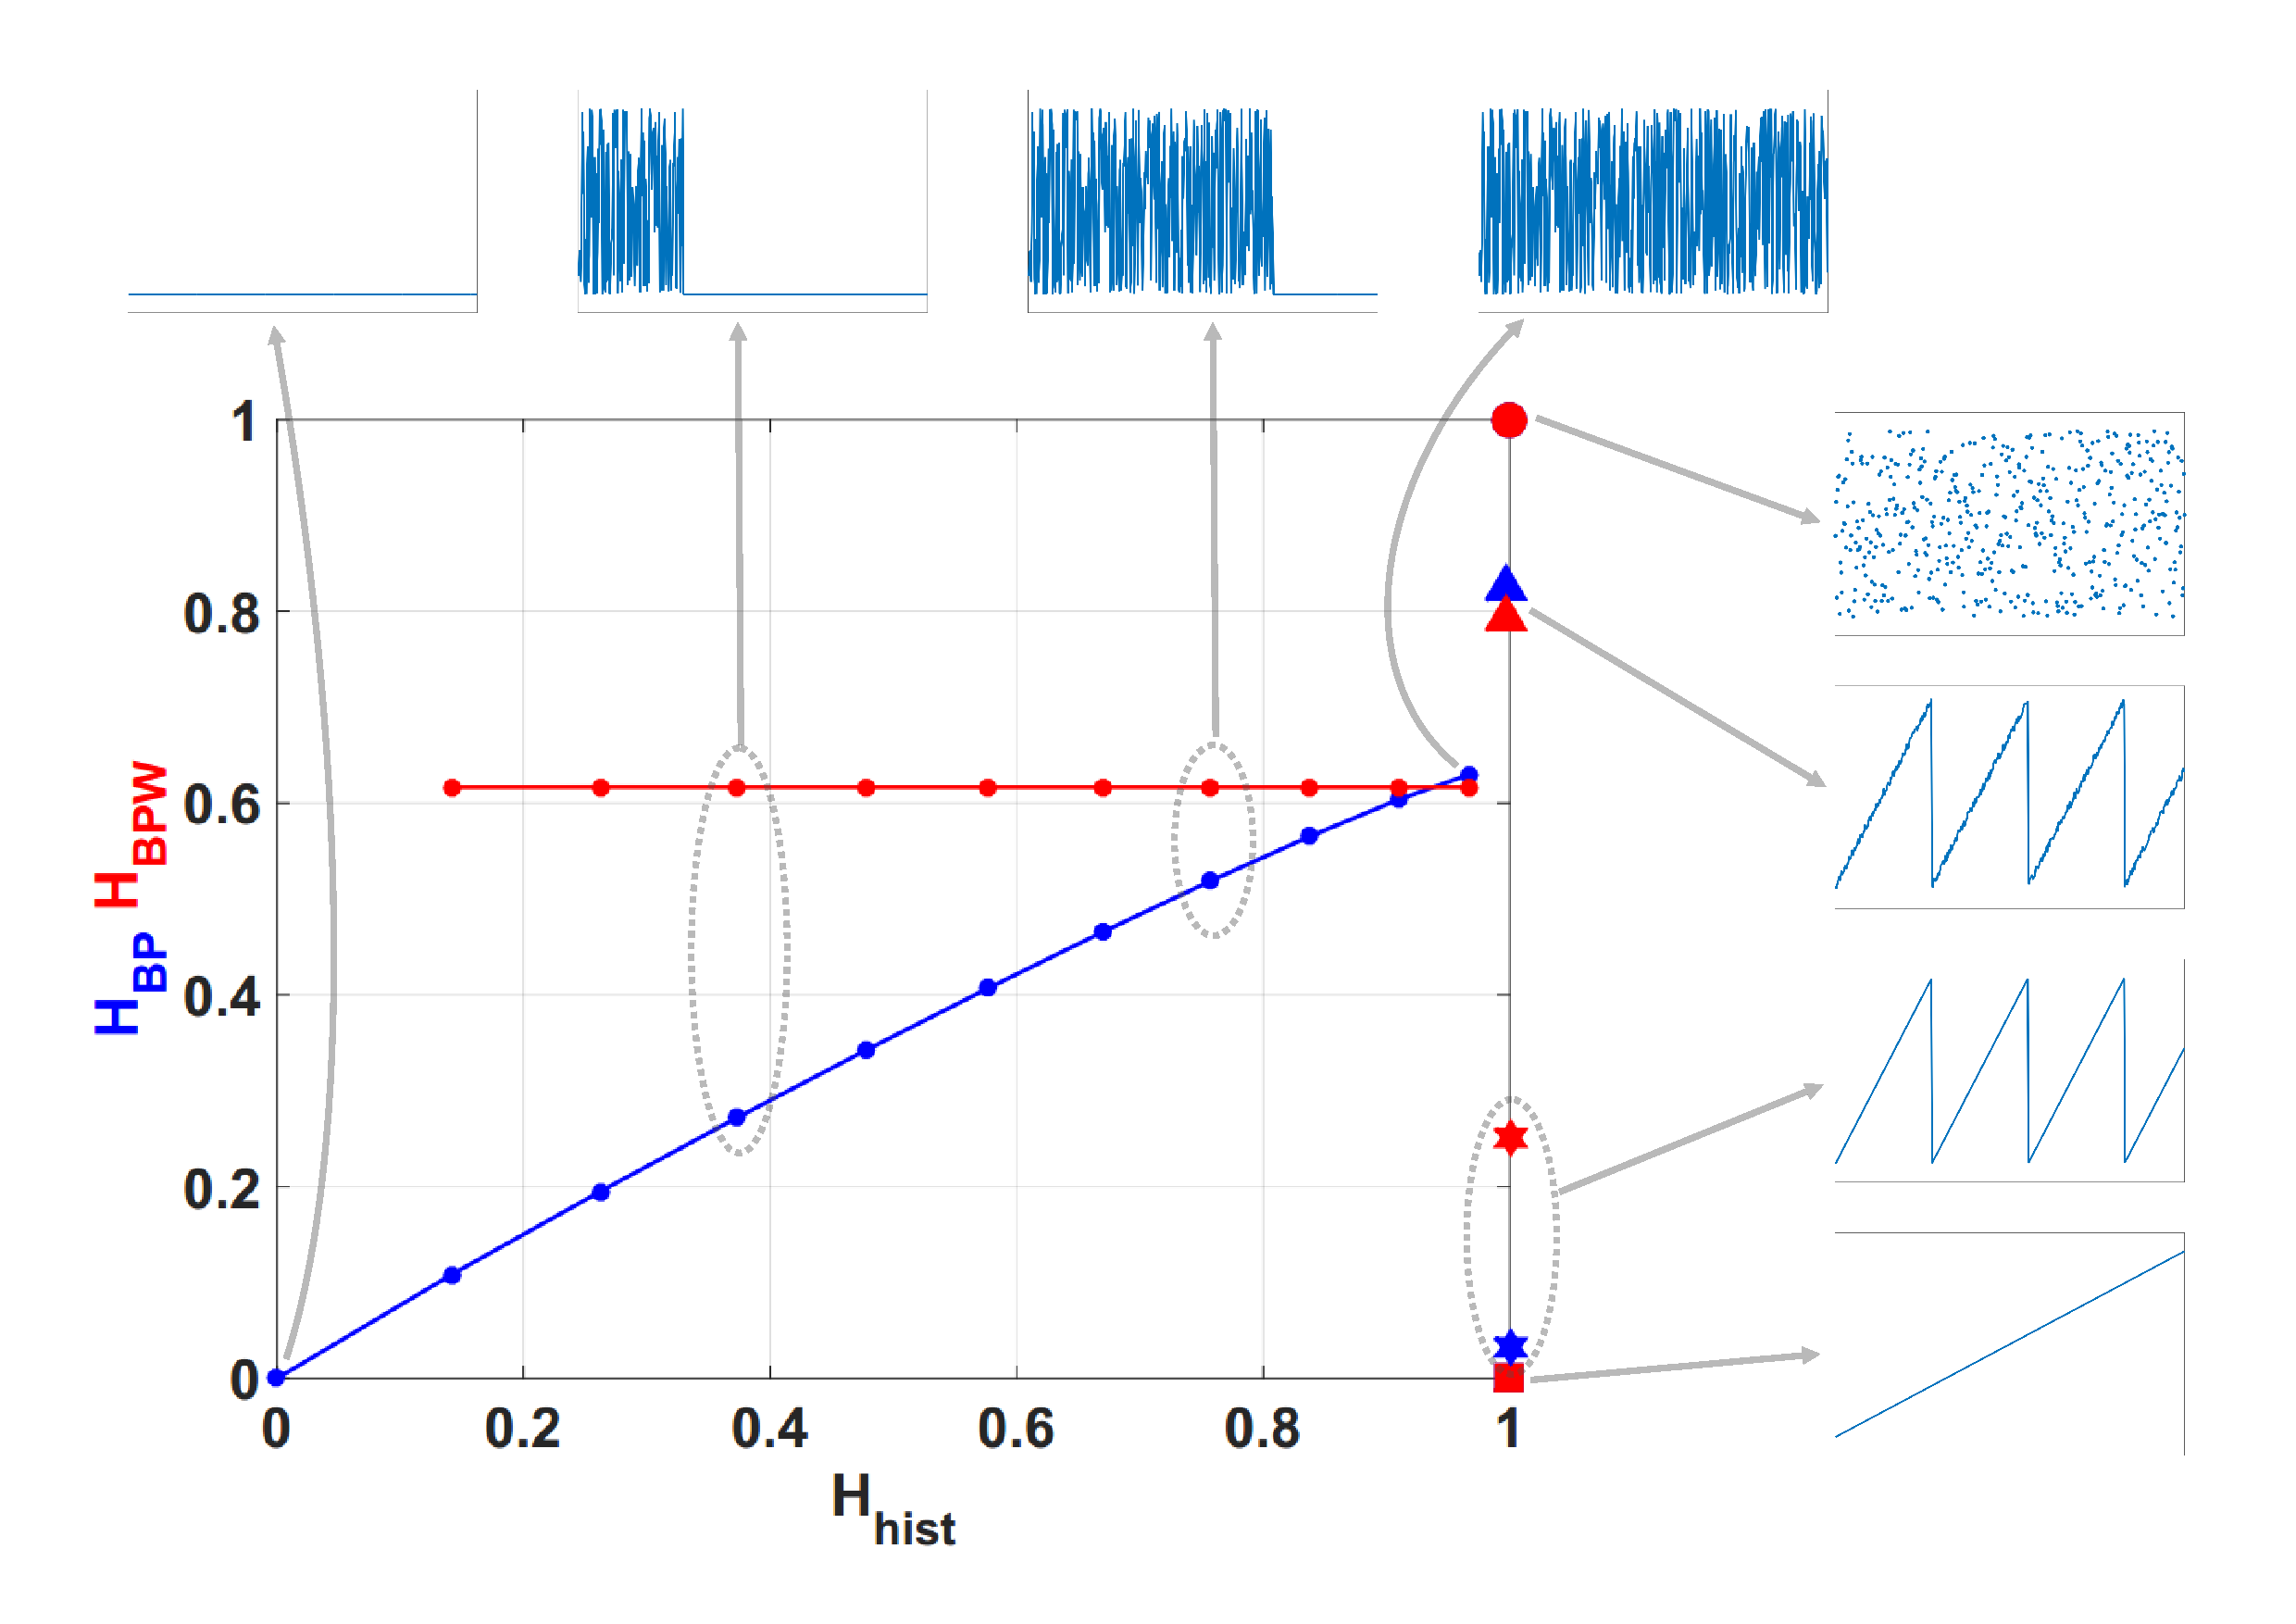
\includegraphics[width= \textwidth]{Fig1HHSignals}
	\caption{Causal-Non causal Entropy plane, values of the quantifiers for some characteristic signals, from purely deterministic through purely random (see text).}
	\label{fig:HH}
\end{figure}

Blue and red stars show $(H_{hist}, H_{BP})$ and $(H_{hist}, H_{BPW})$ respectively, applied to a sawtooth signal.
Values are perfectly distributed in all interval but only a few ordering patterns appear, this explains the high $H_{hist}$ and low $H_{BP}$.
The frequency of occurrence of low amplitude patterns is higher than the one of high amplitude patterns, then the PDF with amplitude contributions is more uniform and $H_{BPW}$ is a little higher than $H_{BP}$.
When sawtooth signal is contaminated with white noise $H_{BP}$ and $H_{BPW}$ are increased as shown with blue and red triangles.
Clearly, new ordering patterns appear and both $H_{BP}$ and $H_{BPW}$ show higher values than non-contaminated case.
However the growth of $H_{BPW}$ is smaller than $H_{BP}$ showing that the technique of recording amplitude contributions adds some immunity to noise.

Finally, we evaluated the quantifiers for a sequence of a logistic map that converges to a fixed point, in all cases the length of data vector remains constant and the length of transitory is variable.
Results obtained without amplitude contributions are depicted in blue dots, they converge to $(H_{hist}, H_{BP})=(0, 0)$ as the length of transitory is shorter, however $H_{BPW}$ (in red points) remains constant for all the cases.
The last point in $(H_{hist}, H_{BP})=(0, 0)$ corresponds to a vector of zeros, in this case the histogram of ordering patterns with amplitude contributions is also a zero vector and $H_{BPW}$ can not be calculated.
Through this last example, we show that the convergence to a fixed point can be detected by the join information of $H_{BP}$ and $H_{BPW}$.

In Figure \ref{fig:HC} we show the causality plane $H_{BP} \times C_{BP}$ with and without amplitude contributions.
The same sample points are showed to illustrate the planar positions for different data vectors.
We can see that not the entire region $0<H_{BP}<1$, $0<C_{BP}<1$ is achievable, in fact, for any PDF the pairs $(H,C)$ of possible values fall between two extreme curves in the plane $H_{BP} \times C_{BP}$ \cite{Anteneodo1996}.
\begin{figure}[H]
	\centering		
	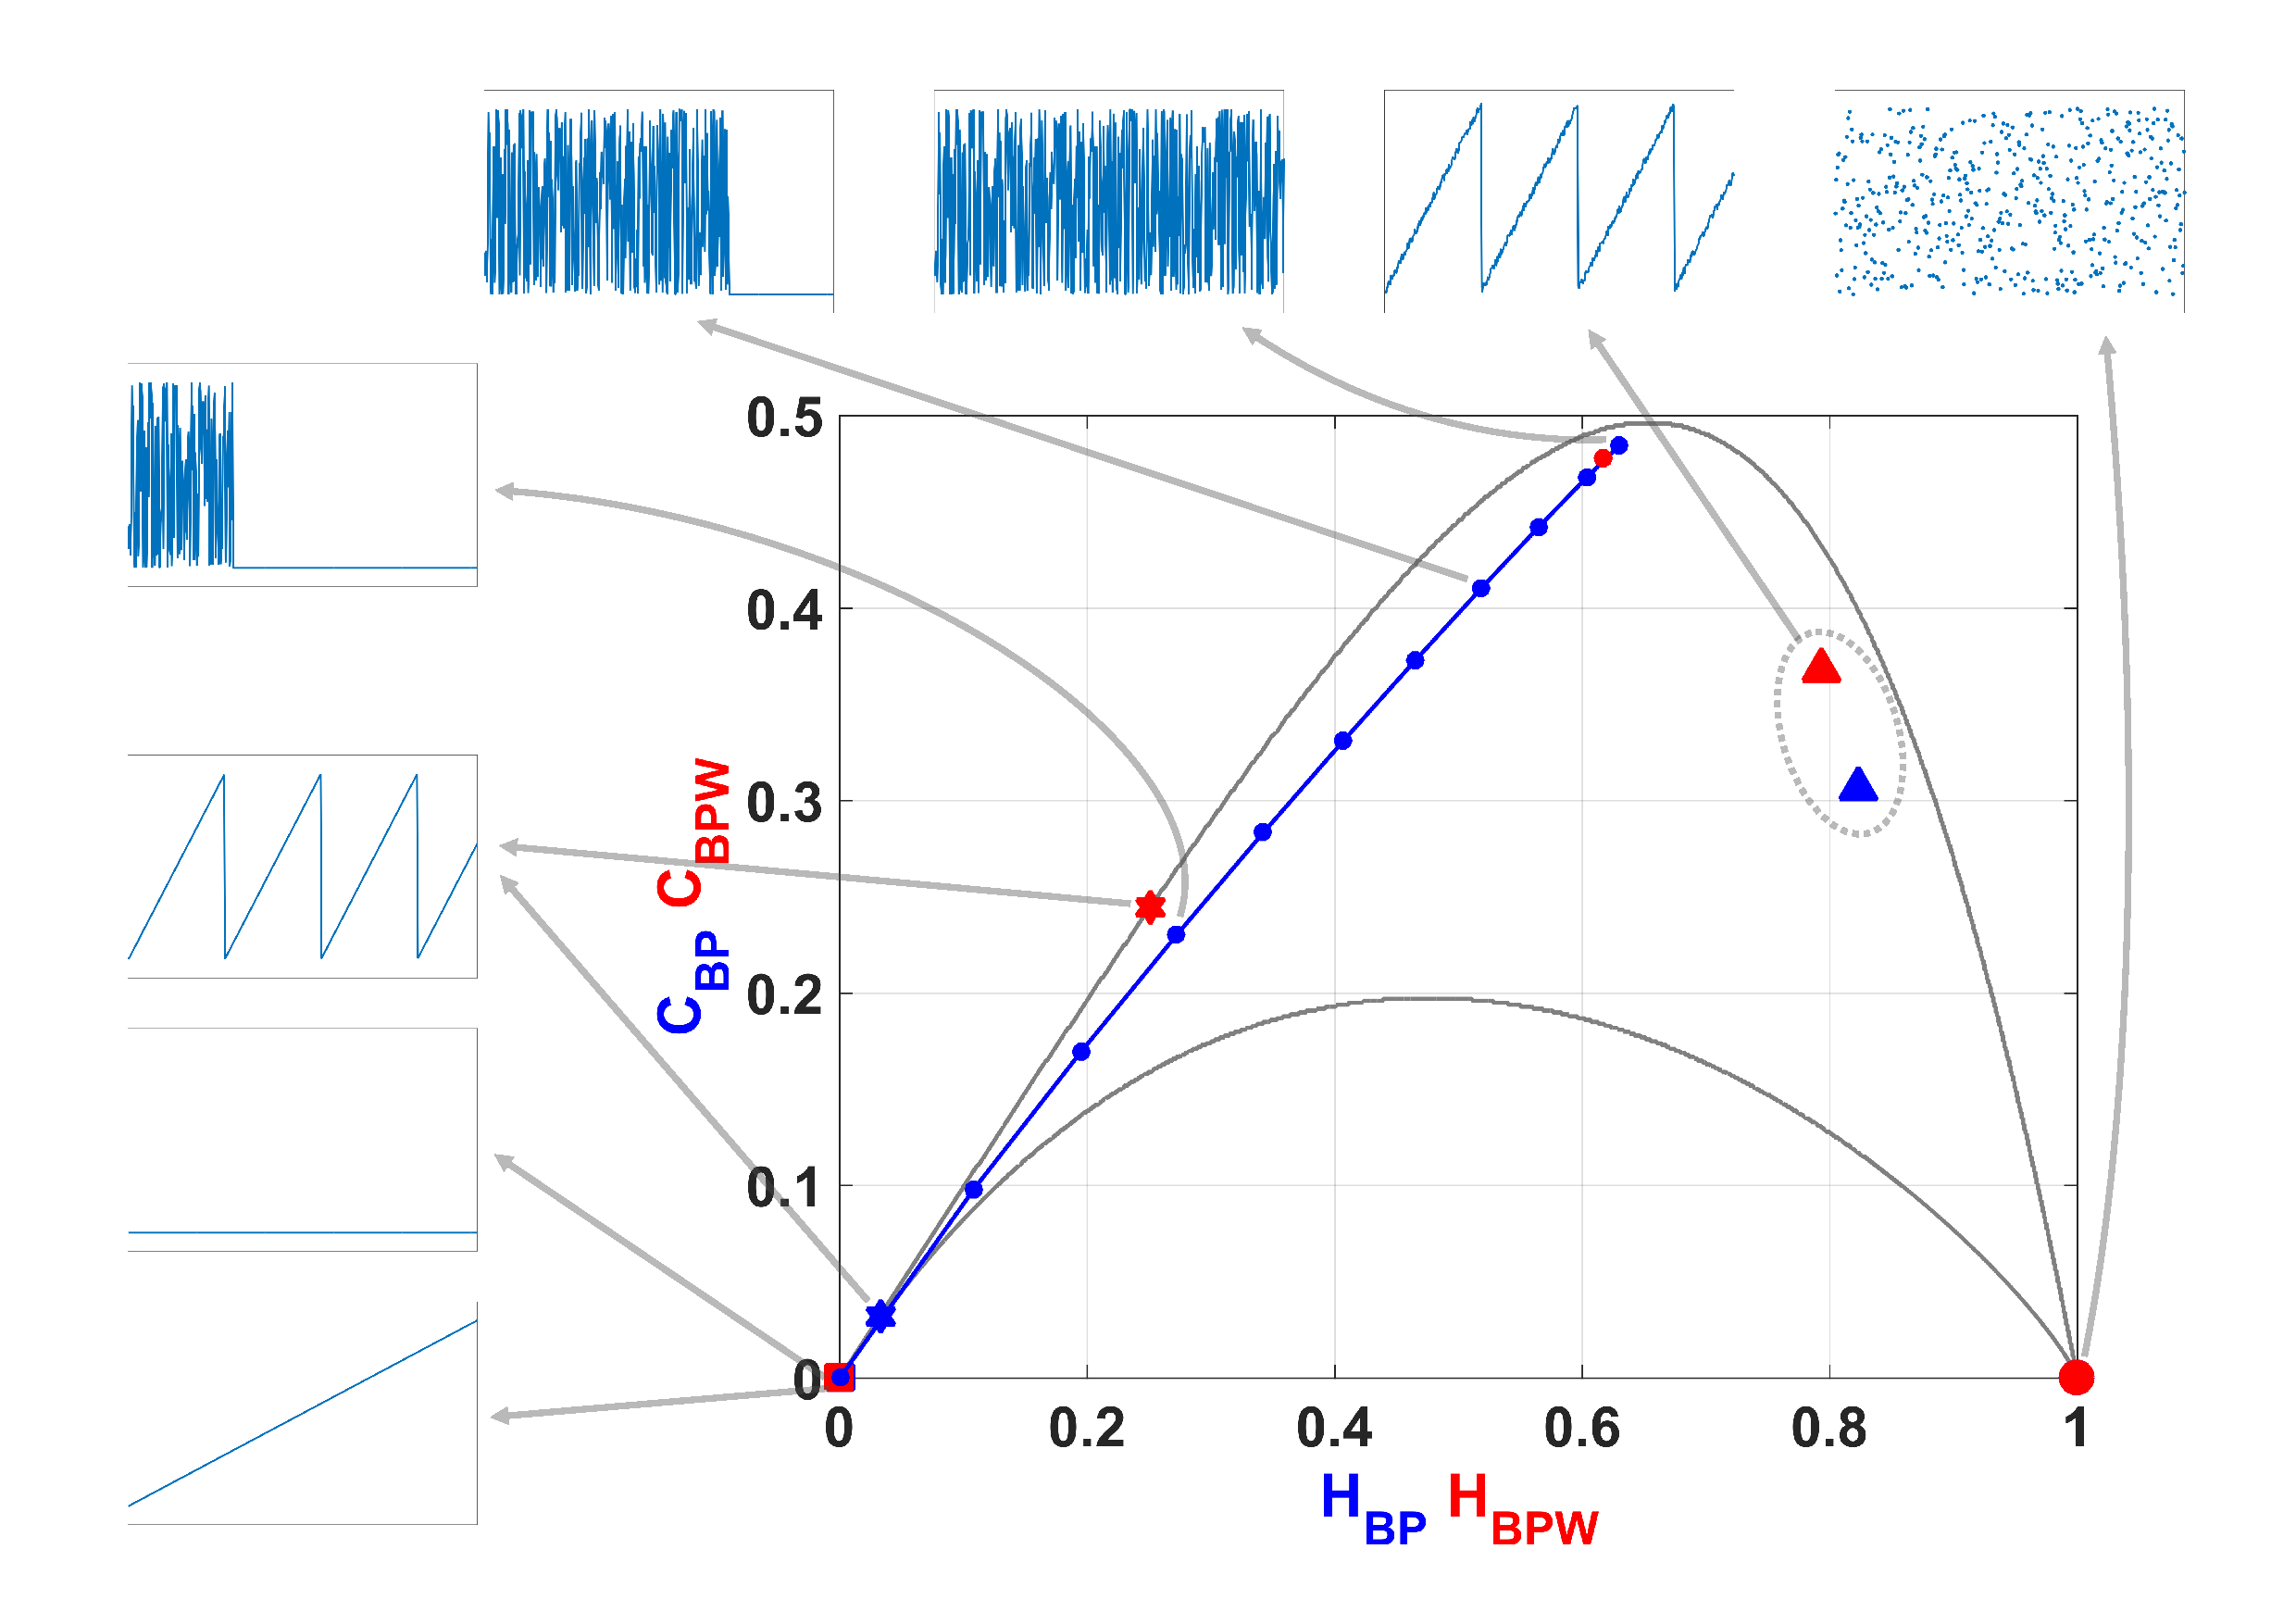
\includegraphics[width= \textwidth]{Fig1HCSignals}
	\caption{Causal Entropy-Complexity plane, values of the quantifiers for some characteristic signals, from purely deterministic trougth purely random (see text).}
	\label{fig:HC}
\end{figure}

Chaotic maps present high values of complexity $C_{BP}$ (close to the upper complexity limit),and intermediate entropy $H_{BP}$ \cite{Rosso2007a,Olivares2012}.
In the case of regular processes the values of entropy and complexity are close to zero. 
Stochastic processes that are uncorrelated present $H_{BP}$ near one and $C_{BP}$ near zero.
Ideal random systems having uniform Bandt \& Pompe PDF, are represented by the point $(1,0)$ \cite{Gonzalez2005} and a delta-like PDF corresponds to the point $(0,0)$.
In both information planes $H_{BP} \times H_{hist}$ in Figure \ref{fig:HH} and $H_{BP} \times C_{BP}$ in Figure \ref{fig:HC}, stochastic, chaotic and deterministic data are clearly localized at different planar positions.

We also used the number of missing patterns MP as a quantifier \cite{Rosso2012}.
As shown recently by Amig\'o {\it et al.} \cite{Amigo2006,Amigo2007,Amigo2008,Amigo2010}, in the case of deterministic maps, not all the possible ordinal patterns can be effectively materialized into orbits.
Thus, for a fixed pattern-length (embedding dimension $D$) the number of missing patterns of a time series (unobserved patterns) is independent of the series length $N$.
Remark that this independence does not characterize other properties of the series such as proximity and correlation, which die out with time \cite{Amigo2007,Amigo2010}.
In this paper, we use the MP to calculate an upper bound to the $H_{BP}$ and $H_{BPW}$.

A complete description and discussion about these quantifiers is out of scope of this manuscript.
However, it can be found in \cite{DeMicco2014,DeMicco2008,Rosso2010,Rosso2012,Lopez-Ruiz1995,Martin2006,Wackerbauer1994,Antonelli2016}.